\documentclass[]{article}

\usepackage{graphicx}
\usepackage{booktabs}
\usepackage{adjustbox}


% Title Page
\title{IE5202 Project 2 Report}
\author{Yang Xiaozhou, A0113538}


\begin{document}
\maketitle

\section{Exploratory Data Analysis}

The exchange rate from 1980 to 1995 seems to have experienced three distinct phases with a drastic drop around 1986. The three phases are shown in Fig \ref{fig:jpy_usd_three_peridos}.
%
\begin{figure}[t]
	\centering
	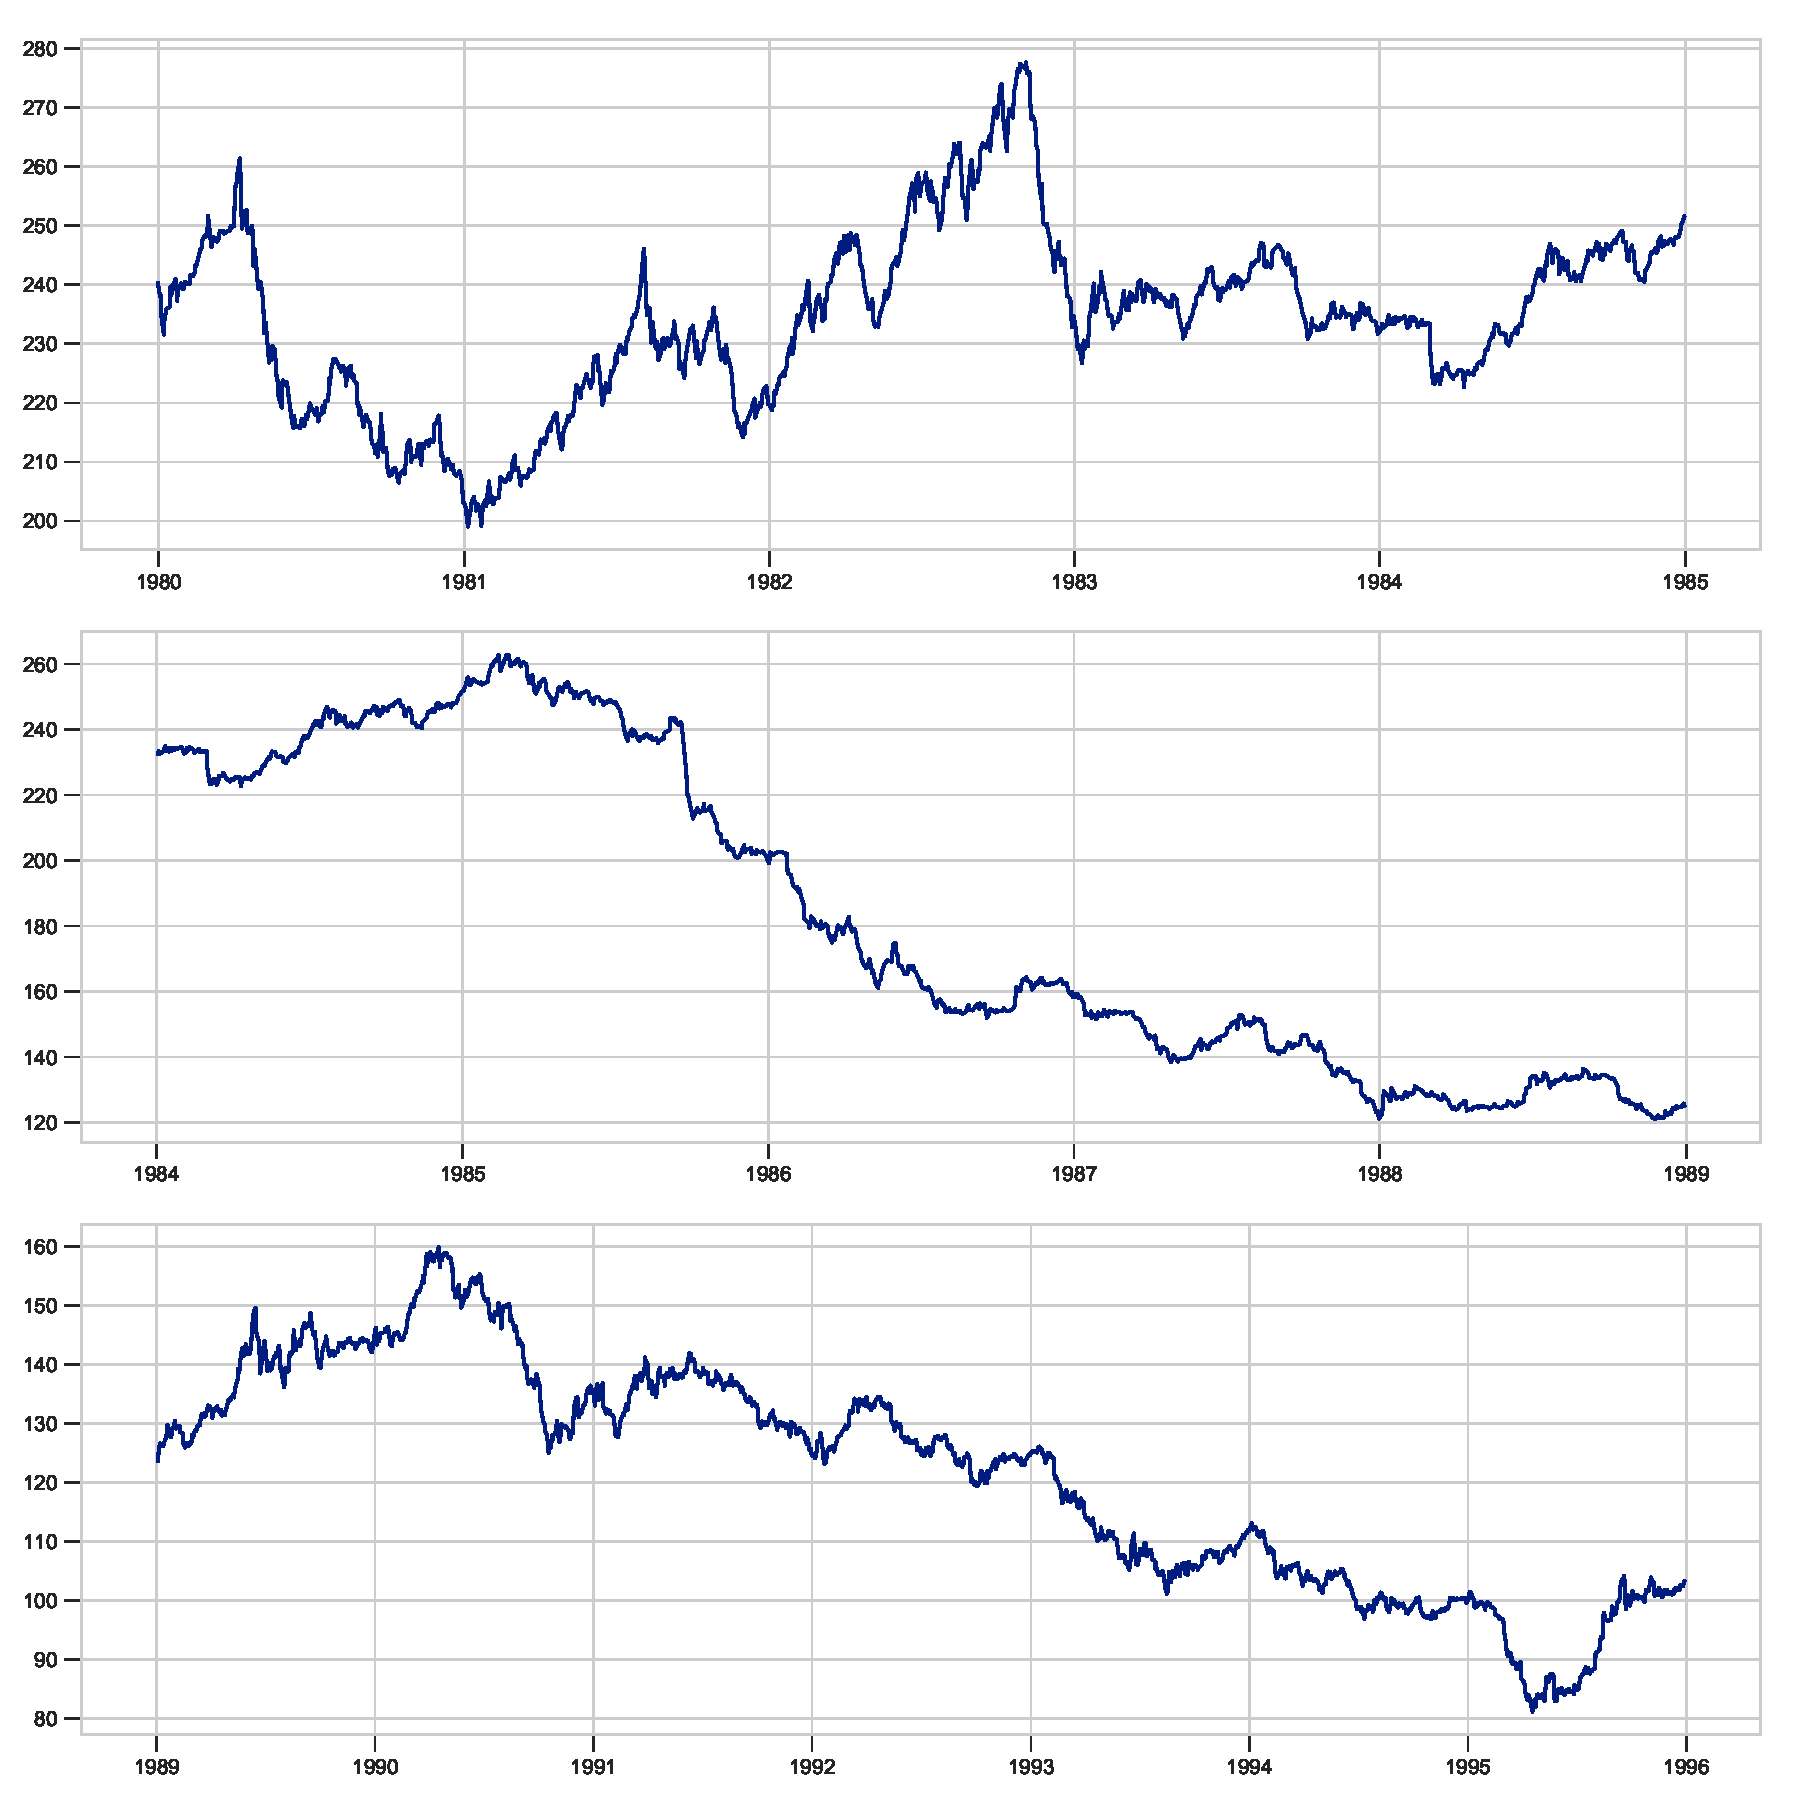
\includegraphics[width=.5\columnwidth]{../Figures/jpy_usd_three_periods.pdf}
	\caption{JPY/USD During Three Separate Periods.}
	\label{fig:jpy_usd_three_peridos}
\end{figure}
%
The time series exhibits strong autocorrelation even beyong 100 lags as shown in Fig \ref{fig:sacf_n_spacf_plot}. SPACF plot shows the lag cuts off after order 1. This indicates an AR(1) model might be appropriate for the time series. 
%
\begin{figure}[ht]
	\centering
	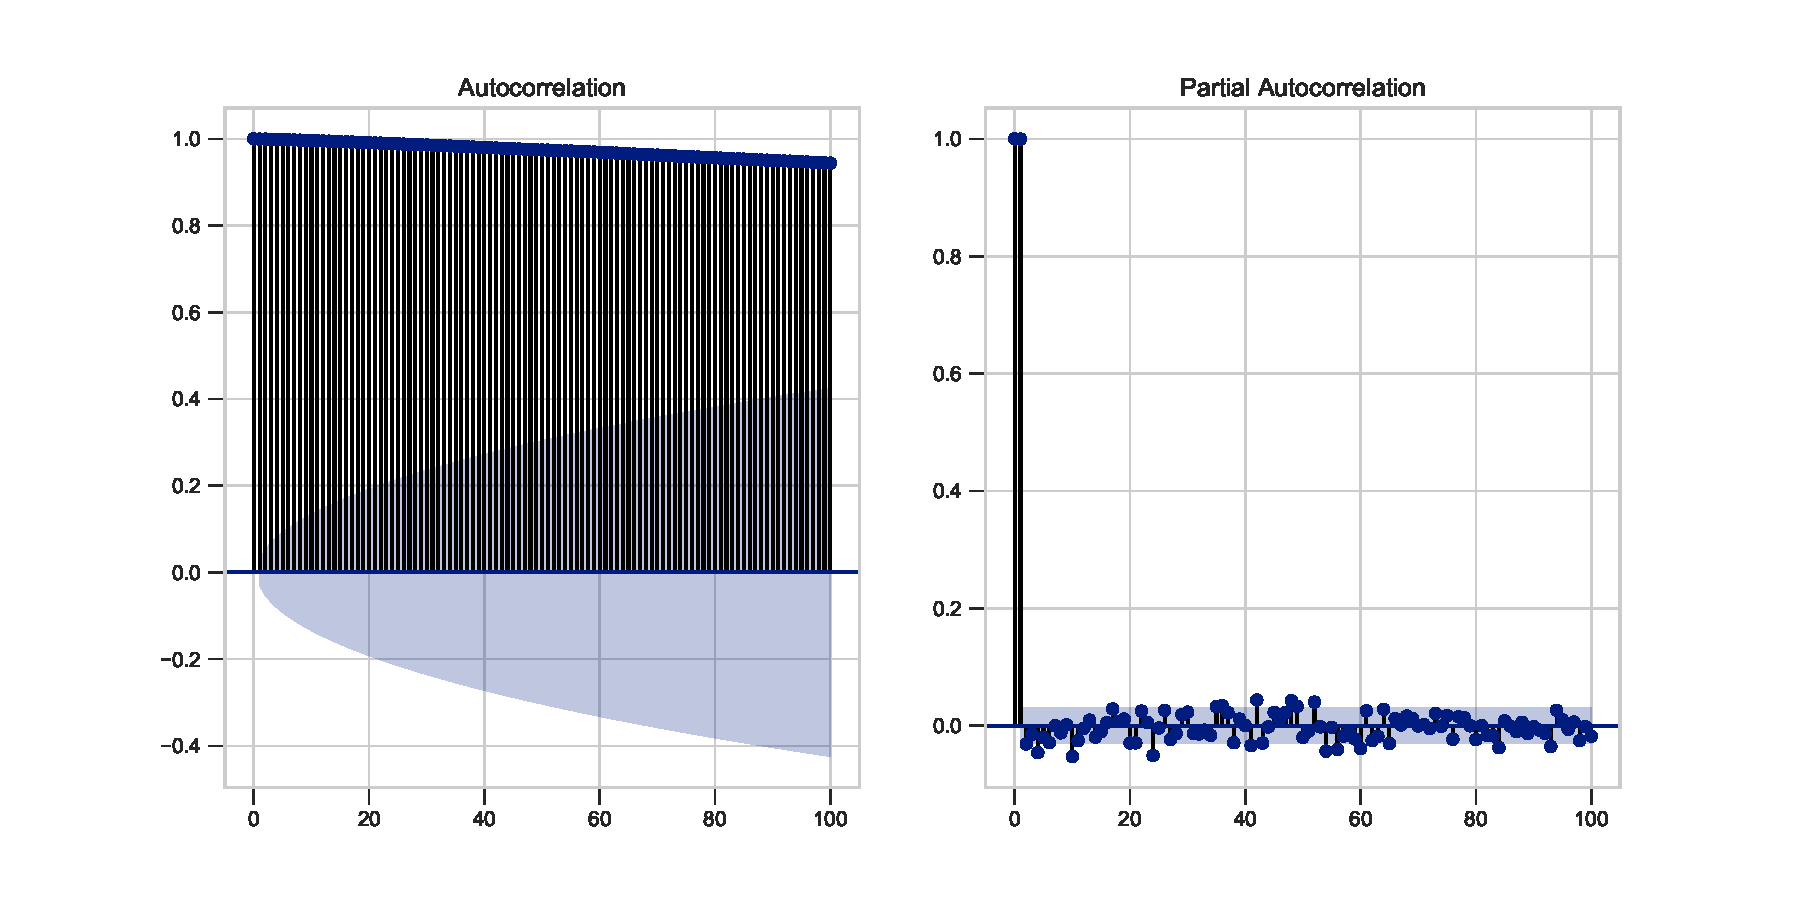
\includegraphics[width=.8\columnwidth]{../Figures/sacf_n_spacf_plot.pdf}
	\caption{SACF and SPACF Plot for JPY/USD.}
	\label{fig:sacf_n_spacf_plot}
\end{figure}
%
Judging from the lag plots in Fig \ref{fig:three_lag_plots}, historical values are very good indicators of the future value, at least in the near future (less than 100 days). 
%
\begin{figure}[ht]
	\centering
	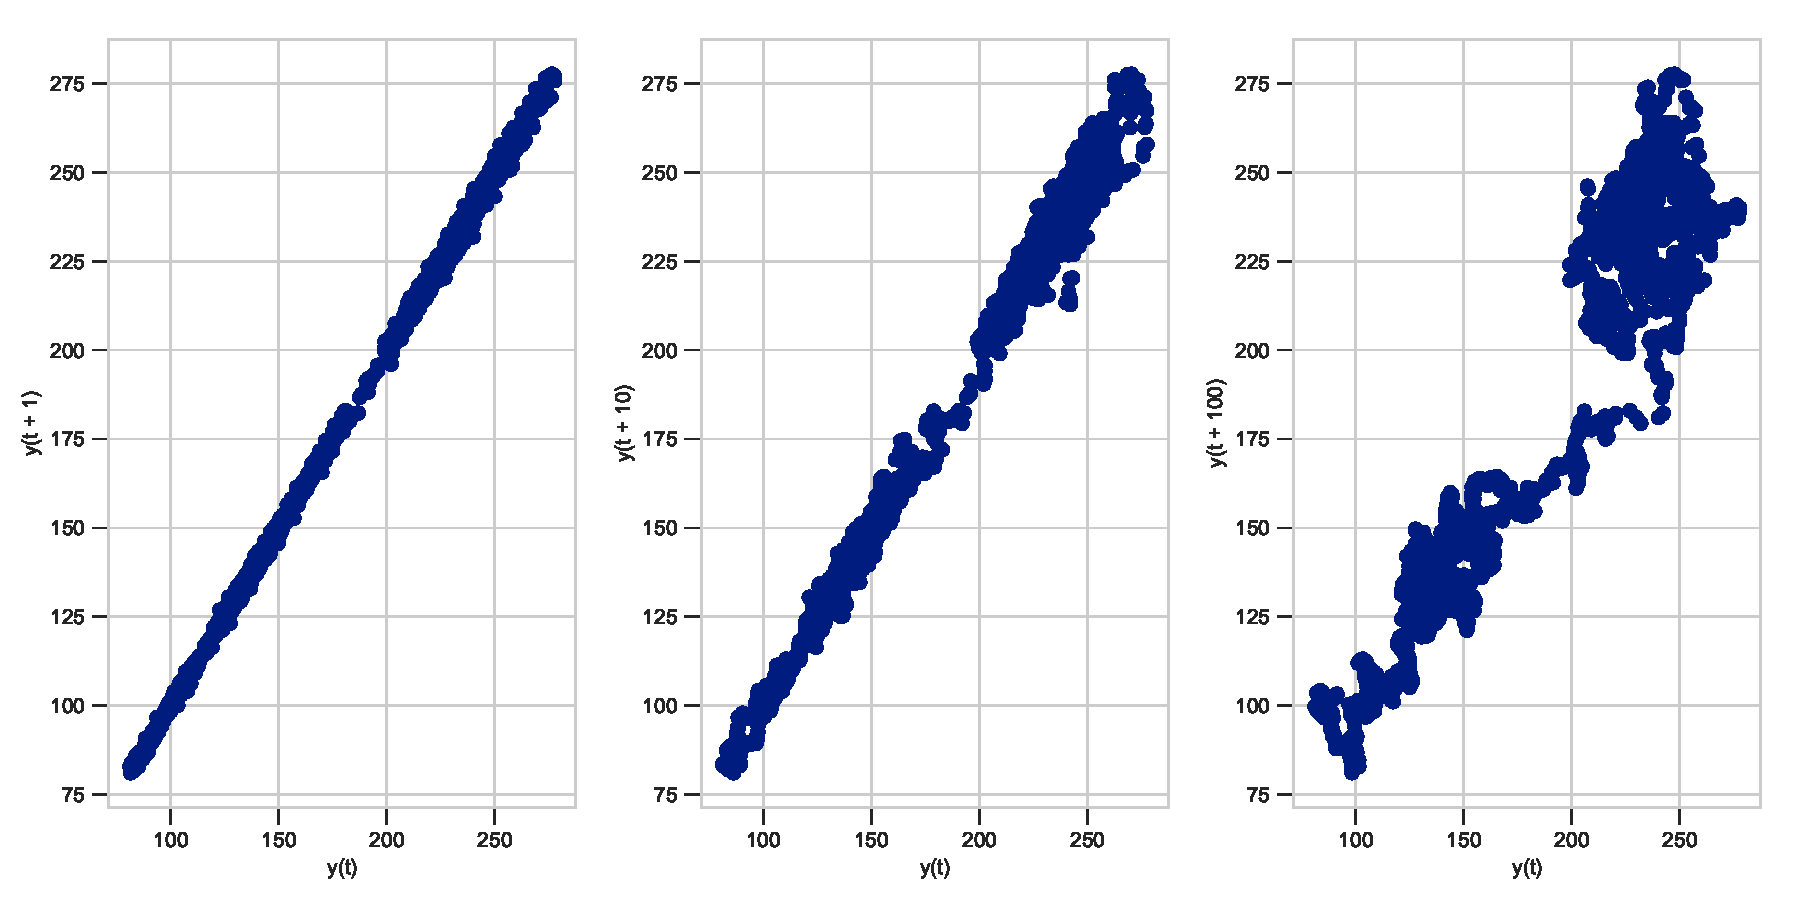
\includegraphics[width=.8\columnwidth]{../Figures/three_lag_plots.pdf}
	\caption{Lag Plots at Three Different Level: 1, 10, 100.}
	\label{fig:three_lag_plots}
\end{figure}
%
Also, no obvious seasonal patterns could be observed. 


\section{Part 1}
\subsection{Exponential Smoothing Model}
With exponentially weighted moving average, due to the strong autocorrelation, the optimal smoothing parameter, alpha, is found to be 1 for the smallest root mean square error (RMSE), see Fig \ref{fig:optimal_alpha_ewma}.
%
\begin{figure}[ht]
	\centering
	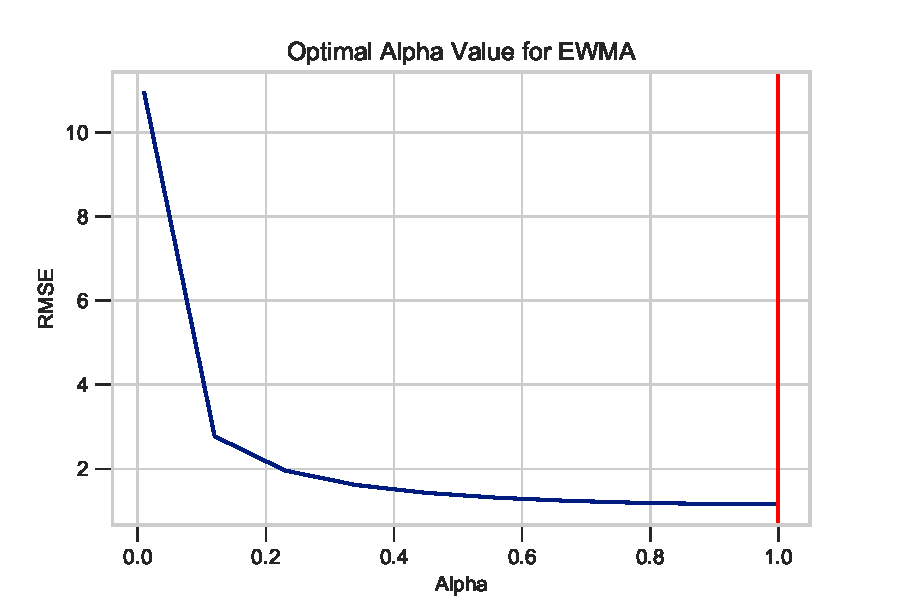
\includegraphics[width=1\columnwidth]{../Figures/optimal_alpha_ewma.pdf}
	\caption{Optimal Alpha.}
	\label{fig:optimal_alpha_ewma}
\end{figure}
%
Similar results are shown when double exponential smoothing model is constructed with the parameter combination of (alpha = 1, beta = 0.12) achieving the least RMSE. 

\subsection{ARIMA Model}
Several ARIMA models are built based on both original data and log-transformed data. 10-fold cross validation RMSEs of 1-step-ahead forecast are reported in Fig \ref{fig:error_estimation_1} for the orginal data and Fig \ref{fig:error_estimation_2} for log-transformed data. For both types of data, AR(1) and MA(1) models on 1st order differencing transformed data perform the best, with the lowest RMSE of 1.048, shown in the two figures as the red horizontal dash lines. This is expected since the foreign exchange rate is a highly autocorrelated time series, hence immediate past values are actually great predictors of the next-day value.

%
\begin{figure}[ht]
	\centering
	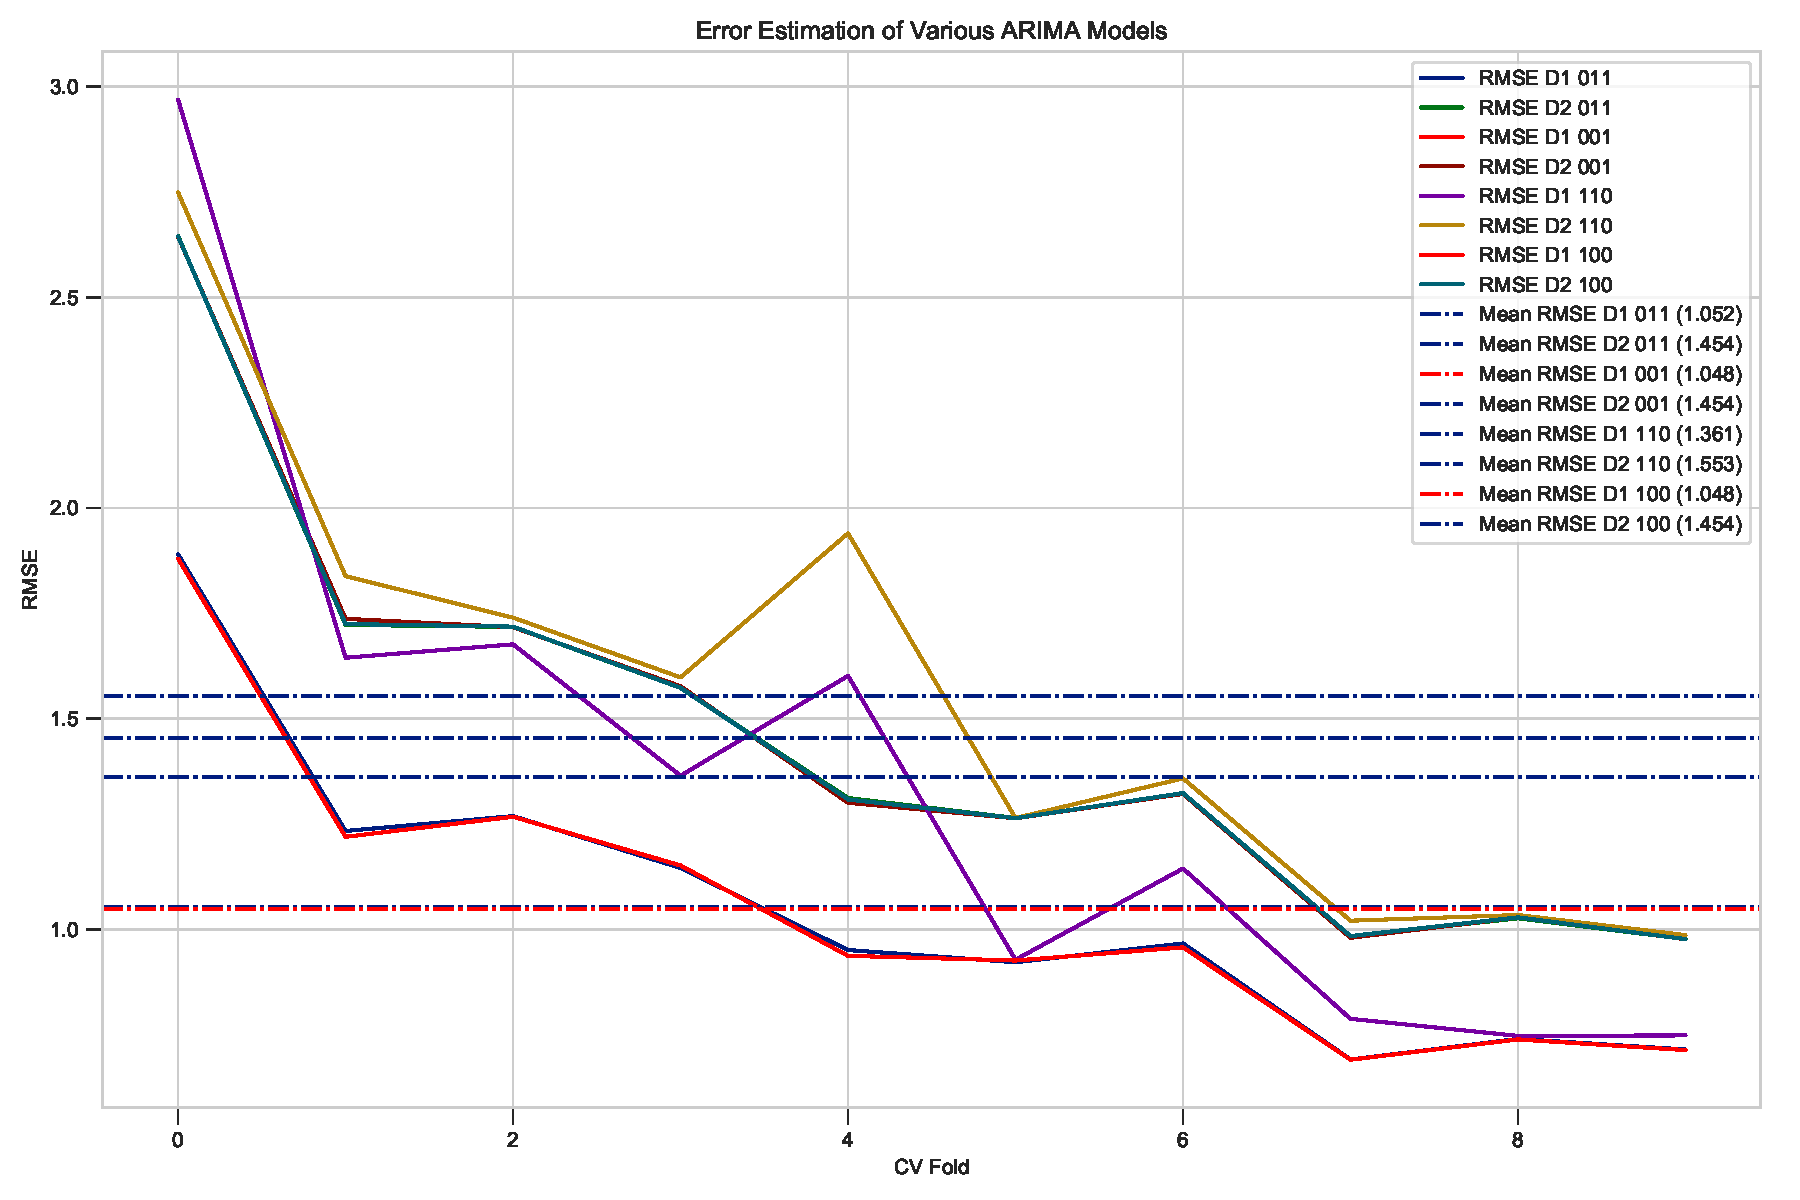
\includegraphics[width=1\columnwidth]{../Figures/error_estimation_1.pdf}
	\caption{Error Estimation on Original Data.}
	\label{fig:error_estimation_1}
\end{figure}
%
%
\begin{figure}[ht]
	\centering
	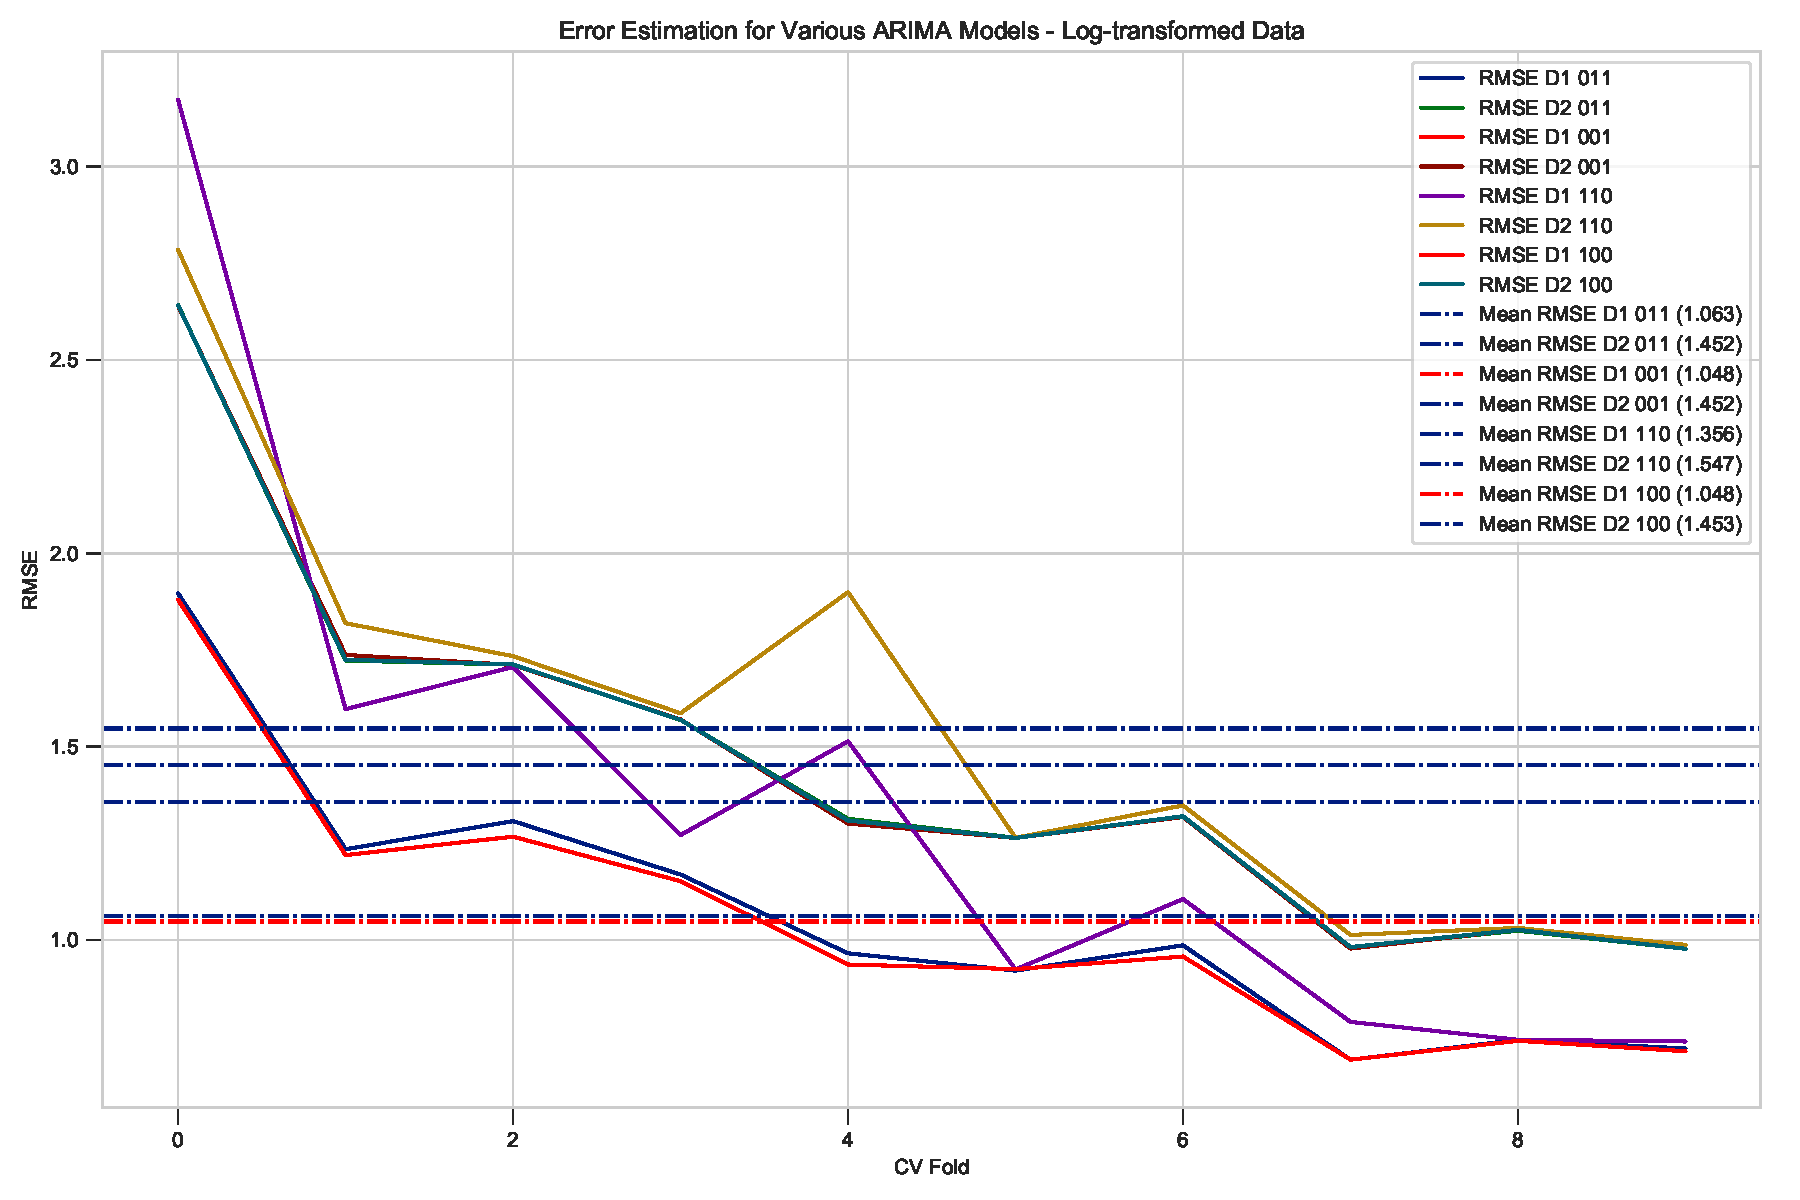
\includegraphics[width=1\columnwidth]{../Figures/error_estimation_2.pdf}
	\caption{Error Estimation on Log-transformed Data.}
	\label{fig:error_estimation_2}
\end{figure}
%

Hence ARIMA(0,1,1) is chosen to model the time series. Since the original data is not stationary, a first order differencing transformation is applied to make it stationary. The resultant time series as shown in Fig \ref{fig:data_1_d} is much more stationary than the original series. Residuals from ARIMA(0,1,1) model are uncorrelated and roughly follow a normal distribution with zero mean, as shown in Fig \ref{fig:res_after_arma} and Fig \ref{fig:sacf_n_spacf_after_arma}. This indicates that ARIMA(0,0,1) is an appropriate model for the time series. 
%
\begin{figure}[ht]
	\centering
	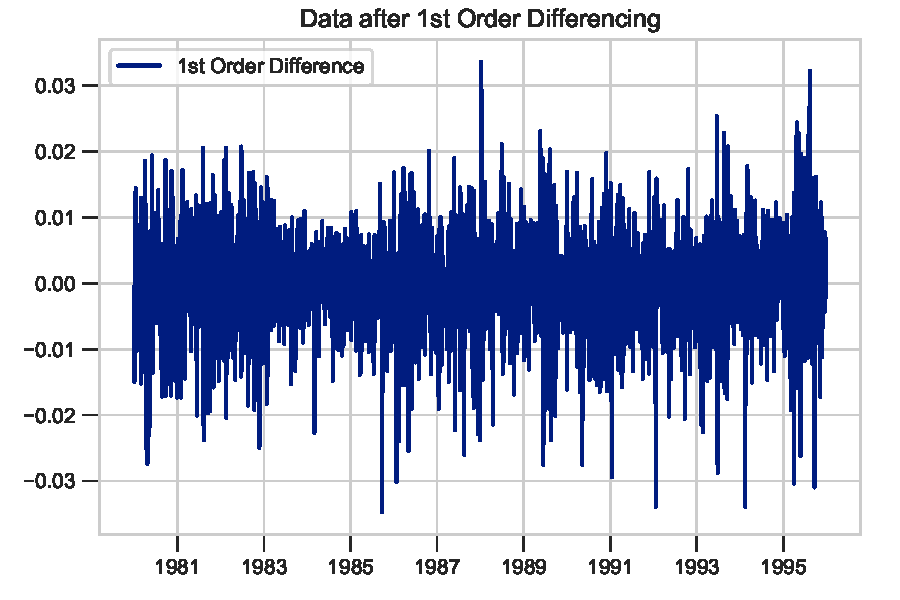
\includegraphics[width=1\columnwidth]{../Figures/data_1_d.pdf}
	\caption{Data after 1st Order Differencing.}
	\label{fig:data_1_d}
\end{figure}
%
%
\begin{figure}[ht]
	\centering
	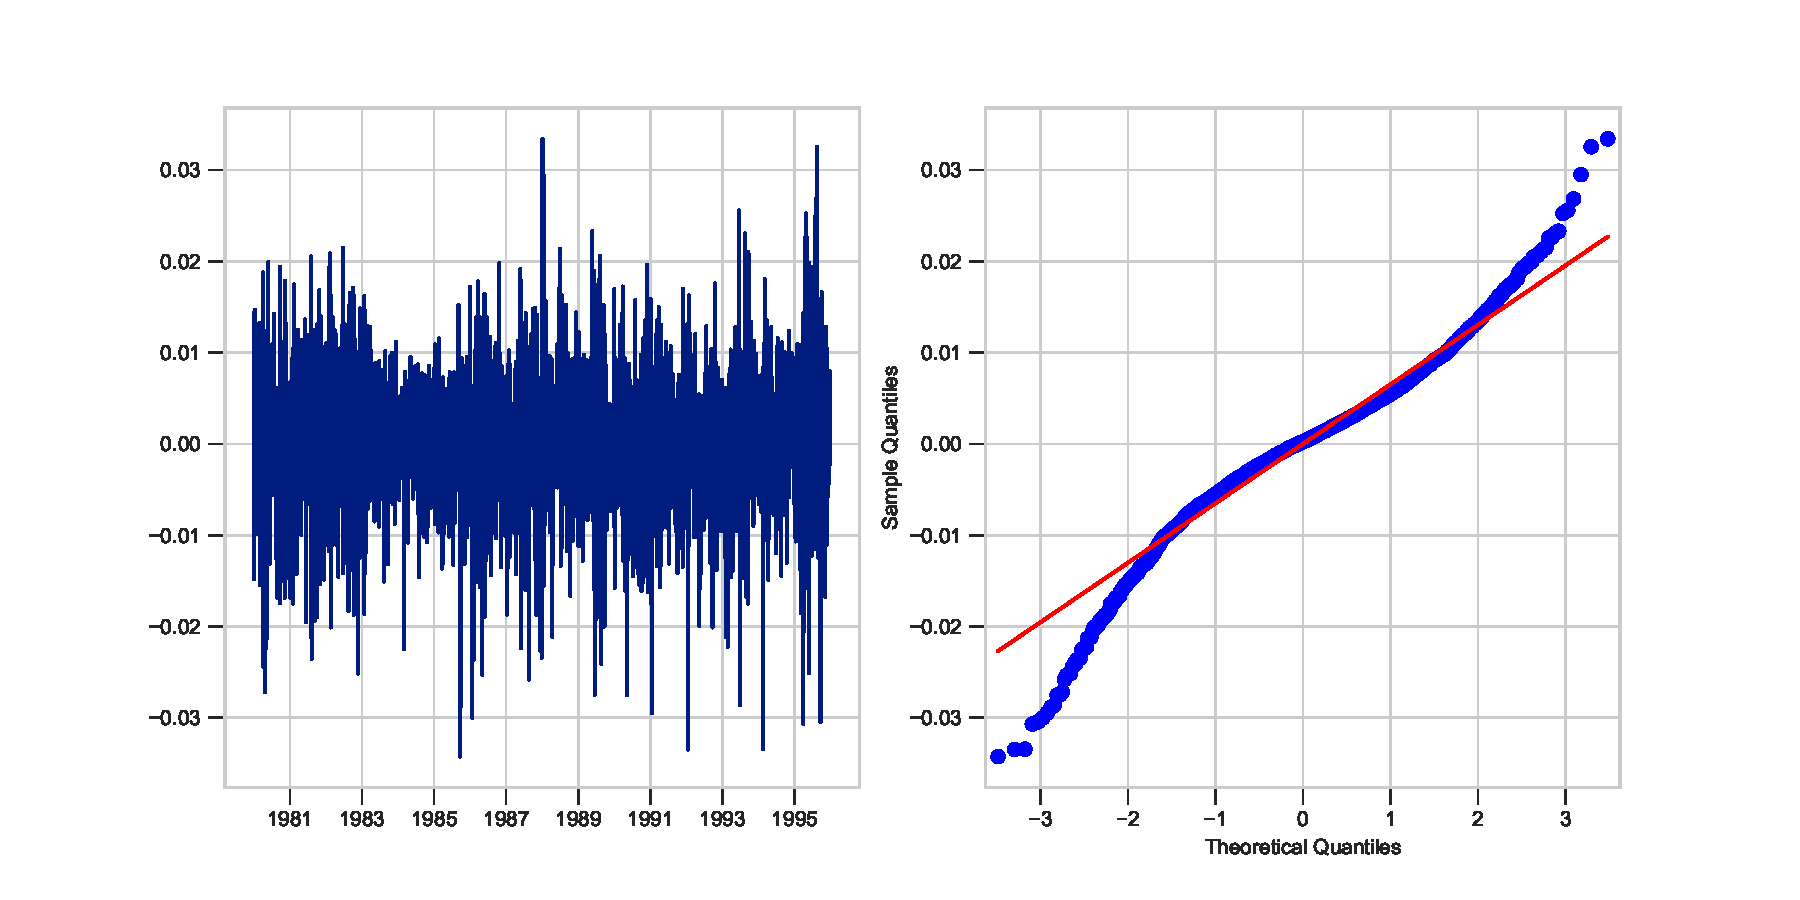
\includegraphics[width=1\columnwidth]{../Figures/res_after_arma.pdf}
	\caption{Residuals of ARIMA(0,1,1) Model.}
	\label{fig:res_after_arma}
\end{figure}
%
%
\begin{figure}[ht]
	\centering
	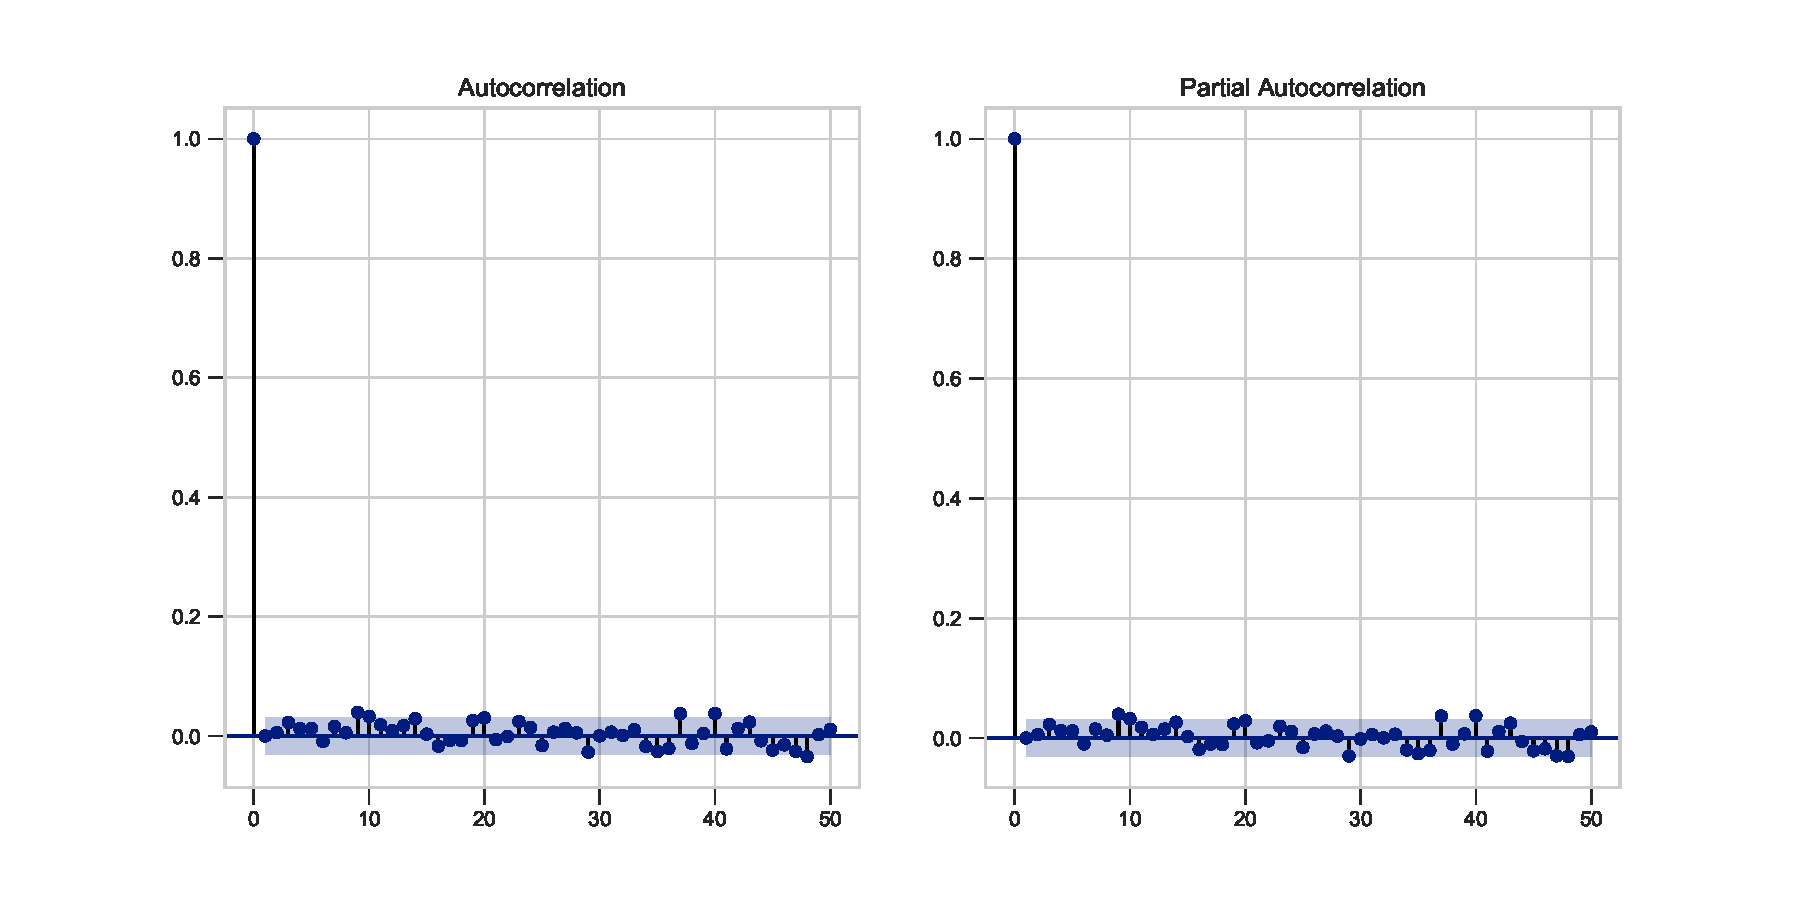
\includegraphics[width=1\columnwidth]{../Figures/sacf_n_spacf_after_arma.pdf}
	\caption{SACF and SPACF of Residuals from ARIMA(0,1,1) Model.}
	\label{fig:sacf_n_spacf_after_arma}
\end{figure}
%

\subsection{Regression on Time}
A least square regression model is developed to model the time series, initially with only time-related information. These include variables of \textit{Year}, \textit{Month}, \textit{Day} and \textit{Day of the Week}. Also, an indicator variable to indicate whether the year is before or after 1986 where the drastic drop happens. However, this regression model does not perform well as the 10-fold cross validation RMSE is a high value of 369. 

Hence, regression based solely on time information is not adequate enough to predict the time series, which is much higher than that of the ARIMA(0,1,1) model. Also, the error is heavily pulled up by the period where the exchange rate declined drastically during 1986. This is expected since the model cannot learn about this drastic drop based on time predictors alone, while ARIMA model allows the model to learn about the drop from the 1st order differencing. Even if the error of that period for regression is omitted, the average RMSE of the rest is still around 24, which is about one-fold higher than that of the ARIMA model.

However, once the regression model has lagged data as one of the predictors, the performance improves tremendously. This can be seen from the error estimation plot of Fig \ref{fig:error_estimation_3} where four different regression models' performance are compared:
\begin{enumerate}
	\item Lag 1: Regression on time information and Lag 1 value
	\item Lag 5: Regression on time information and Lag 5 value
	\item w Lag Diff: Regression on time information, Lag 1 value and the difference between Lag 1 and Lag 2 value
	\item  Lag \& Cat: Regression on only 1986 indicator variable, Lag 1 data and the difference between Lag 1 and Lag 2 data. This is the simplest version among all four models.
\end{enumerate}

As seen from Fig \ref{fig:error_estimation_3}, The fourth model performs the best, obtaining the lowest RMSE of 1.048 wihch is identical as the ARIMA(0,1,1) model. This is not surprising since both models utilized information on Lag 1 data and the difference between previous two values. The whole dataset was fitted with the best regression model and Table \ref{tab:regression_results} reports the regression summary. Each of the model parameters are statistically significant and both R-scores are very high. The residuals of the model seem to be uncorrelated with each other (Fig \ref{fig:sacf_n_spacf_after_reg}) and follows a normal distribution with zero mean (Fig \ref{fig:res_after_reg}). 

%
\begin{figure}[ht]
	\centering
	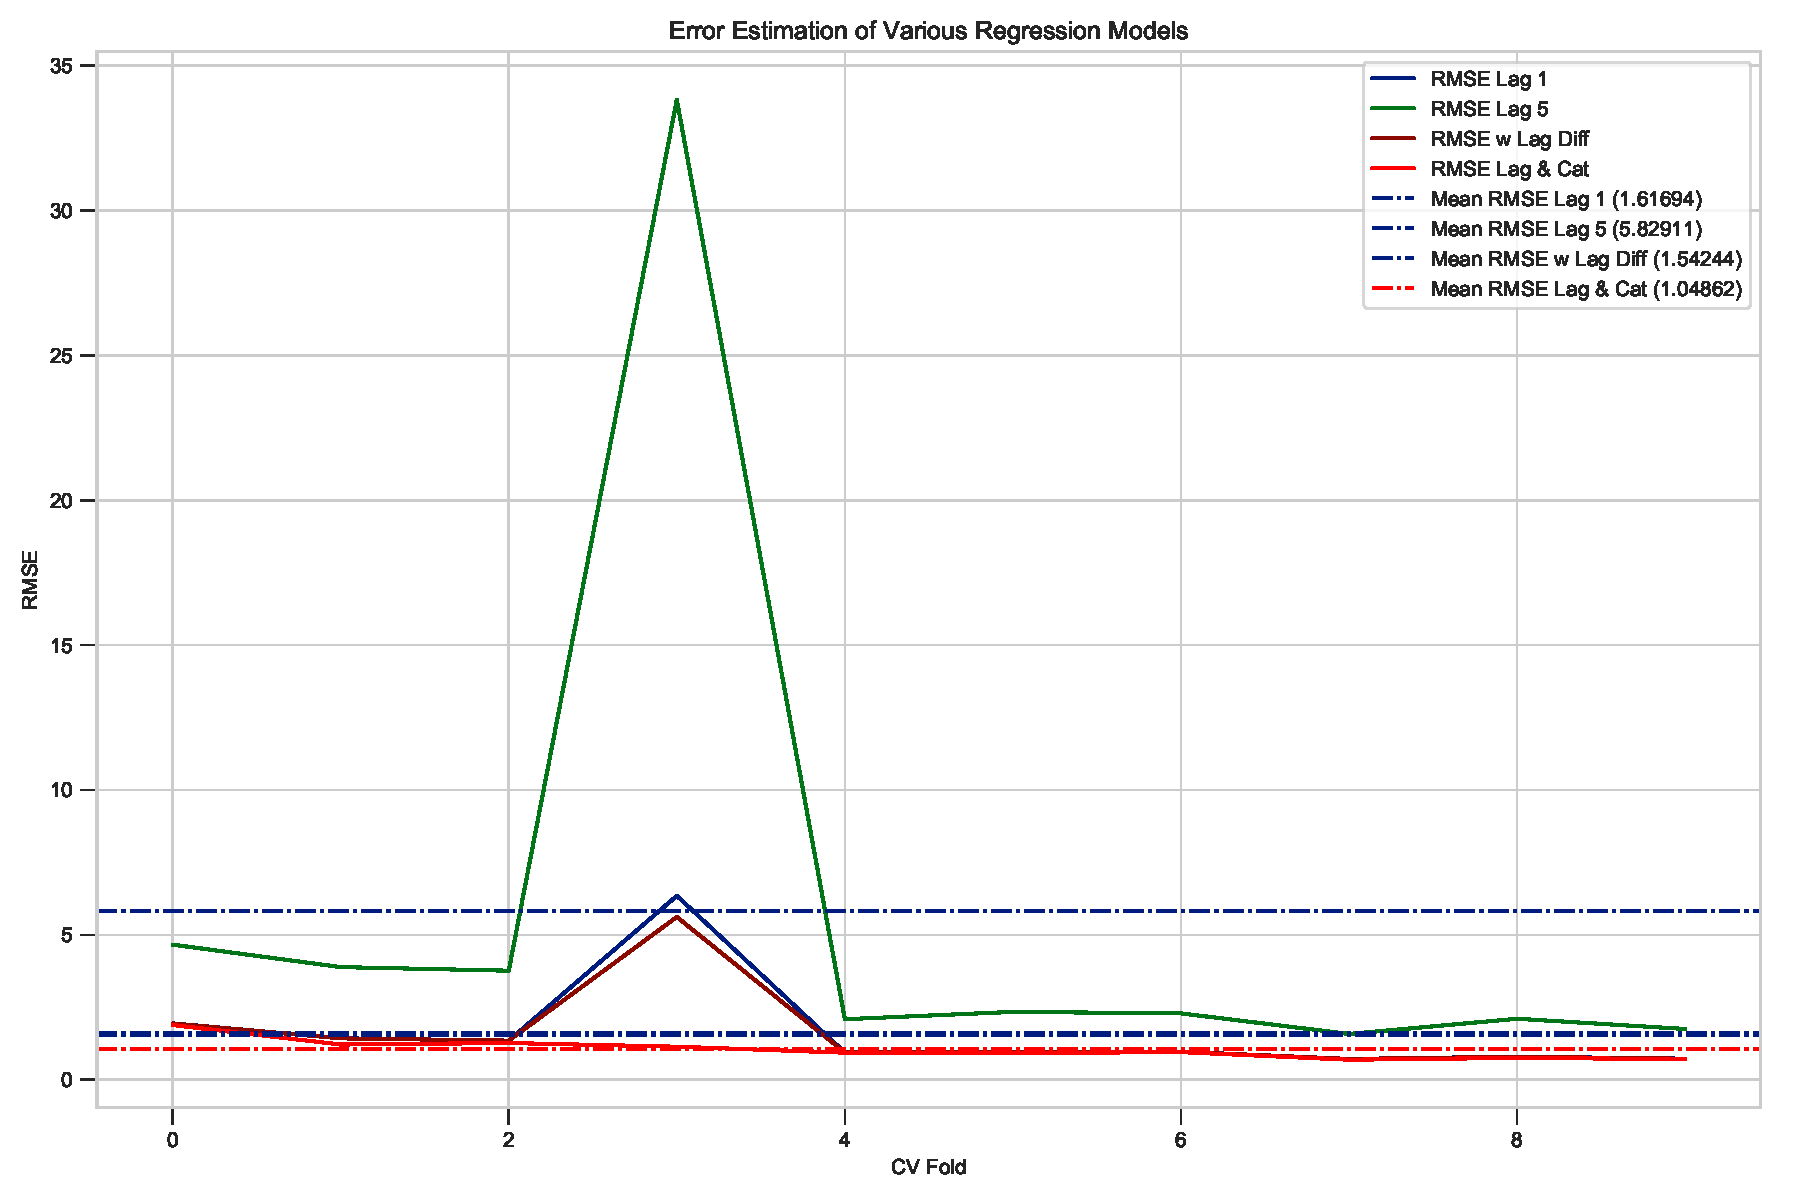
\includegraphics[width=1\columnwidth]{../Figures/error_estimation_3.pdf}
	\caption{Error Estimation of Various Regression Models.}
	\label{fig:error_estimation_3}
\end{figure}
%

\begin{table}
\begin{center}
	\begin{tabular}{lclc}
		\toprule
		\textbf{Dep. Variable:}       &     JPY\_USD      & \textbf{  R-squared:         } &     1.000   \\
		\textbf{Model:}               &       OLS        & \textbf{  Adj. R-squared:    } &     1.000   \\
		\textbf{Method:}              &  Least Squares   & \textbf{  F-statistic:       } & 3.032e+06   \\
		\textbf{Date:}                & Sun, 19 Nov 2017 & \textbf{  Prob (F-statistic):} &     0.00    \\
		\textbf{Time:}                &     20:57:14     & \textbf{  Log-Likelihood:    } &   -6274.6   \\
		\textbf{No. Observations:}    &        4017      & \textbf{  AIC:               } & 1.256e+04   \\
		\textbf{Df Residuals:}        &        4013      & \textbf{  BIC:               } & 1.258e+04   \\
		\textbf{Df Model:}            &           3      & \textbf{                     } &             \\
		\bottomrule
	\end{tabular}
	\begin{tabular}{lcccccc}
		& \textbf{coef} & \textbf{std err} & \textbf{t} & \textbf{P$>$$|$t$|$} & \textbf{[0.025} & \textbf{0.975]}  \\
		\midrule
		\textbf{Intercept}            &       0.3044  &        0.119     &     2.551  &         0.011        &        0.070    &        0.538     \\
		\textbf{C(bef\_1986)[T.True]} &       0.2920  &        0.103     &     2.840  &         0.005        &        0.090    &        0.494     \\
		\textbf{diff\_lag\_1\_lag\_2} &       0.0316  &        0.016     &     2.004  &         0.045        &        0.001    &        0.062     \\
		\textbf{jpy\_usd\_lag\_1}     &       0.9974  &        0.001     &  1101.504  &         0.000        &        0.996    &        0.999     \\
		\bottomrule
	\end{tabular}
	\begin{tabular}{lclc}
		\textbf{Omnibus:}       & 570.043 & \textbf{  Durbin-Watson:     } &    2.001  \\
		\textbf{Prob(Omnibus):} &   0.000 & \textbf{  Jarque-Bera (JB):  } & 3070.672  \\
		\textbf{Skew:}          &  -0.563 & \textbf{  Prob(JB):          } &     0.00  \\
		\textbf{Kurtosis:}      &   7.132 & \textbf{  Cond. No.          } & 1.49e+03  \\
		\bottomrule
	\end{tabular}

\end{center}
\caption{OLS Regression Results}
\label{tab:regression_results}
\end{table}

%
\begin{figure}[ht]
	\centering
	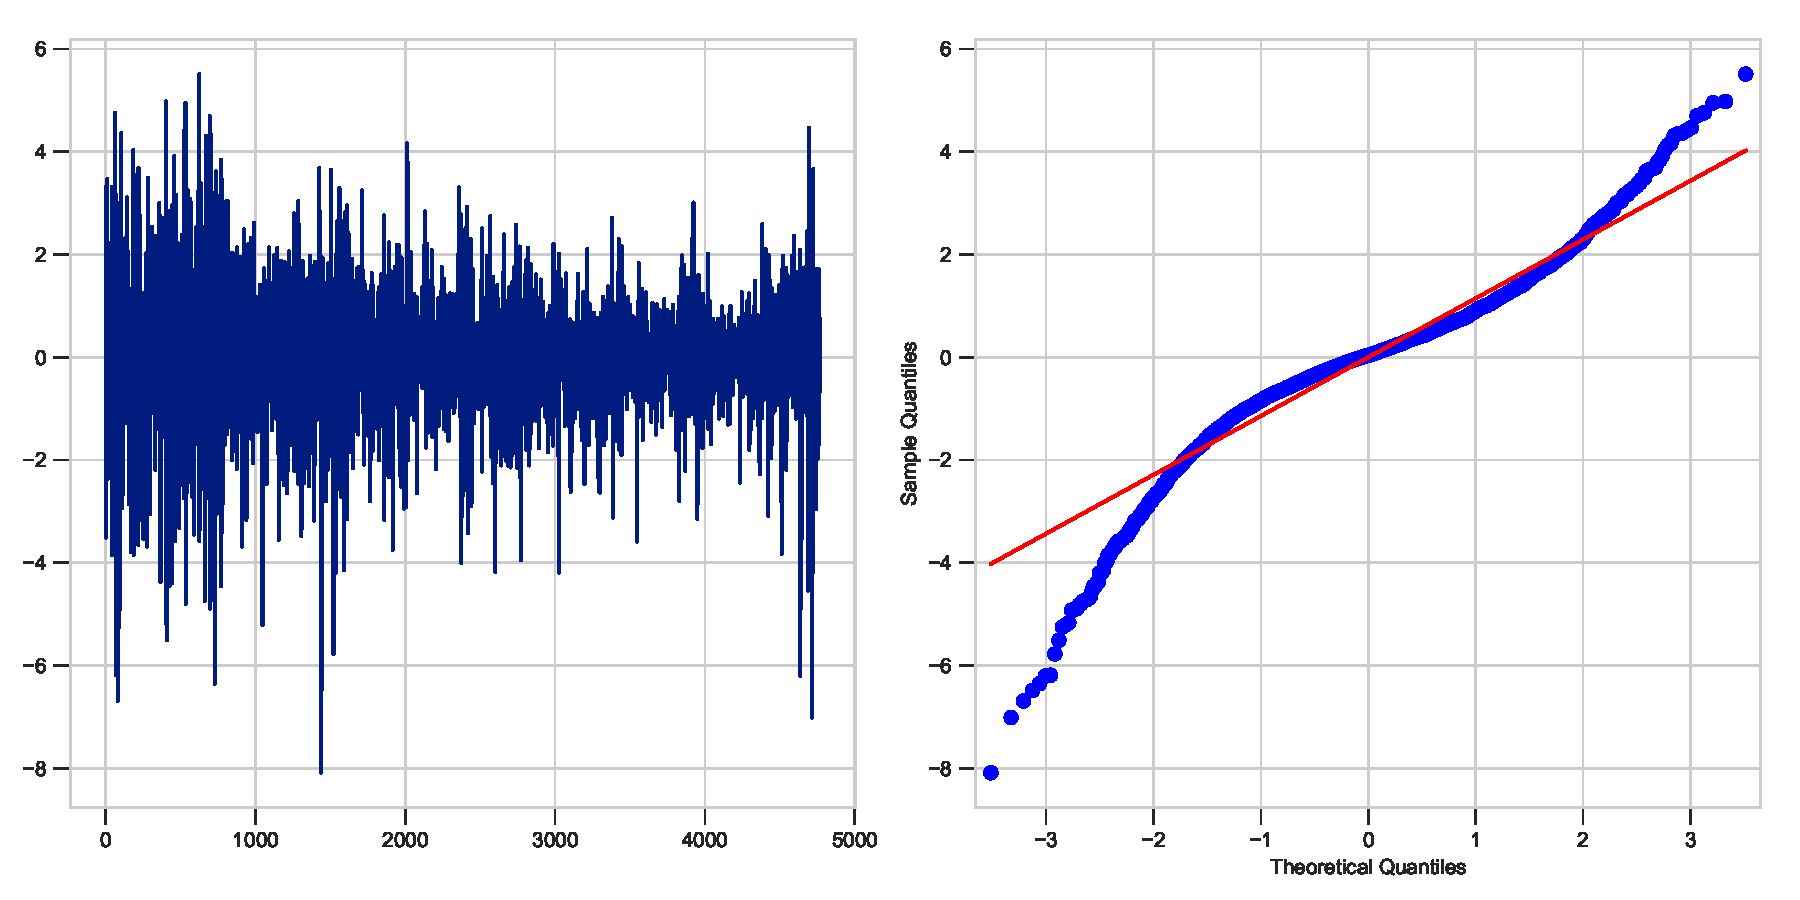
\includegraphics[width=1\columnwidth]{../Figures/res_after_reg.pdf}
	\caption{Residuals of Regression Model.}
	\label{fig:res_after_reg}
\end{figure}
%
%
\begin{figure}[ht]
	\centering
	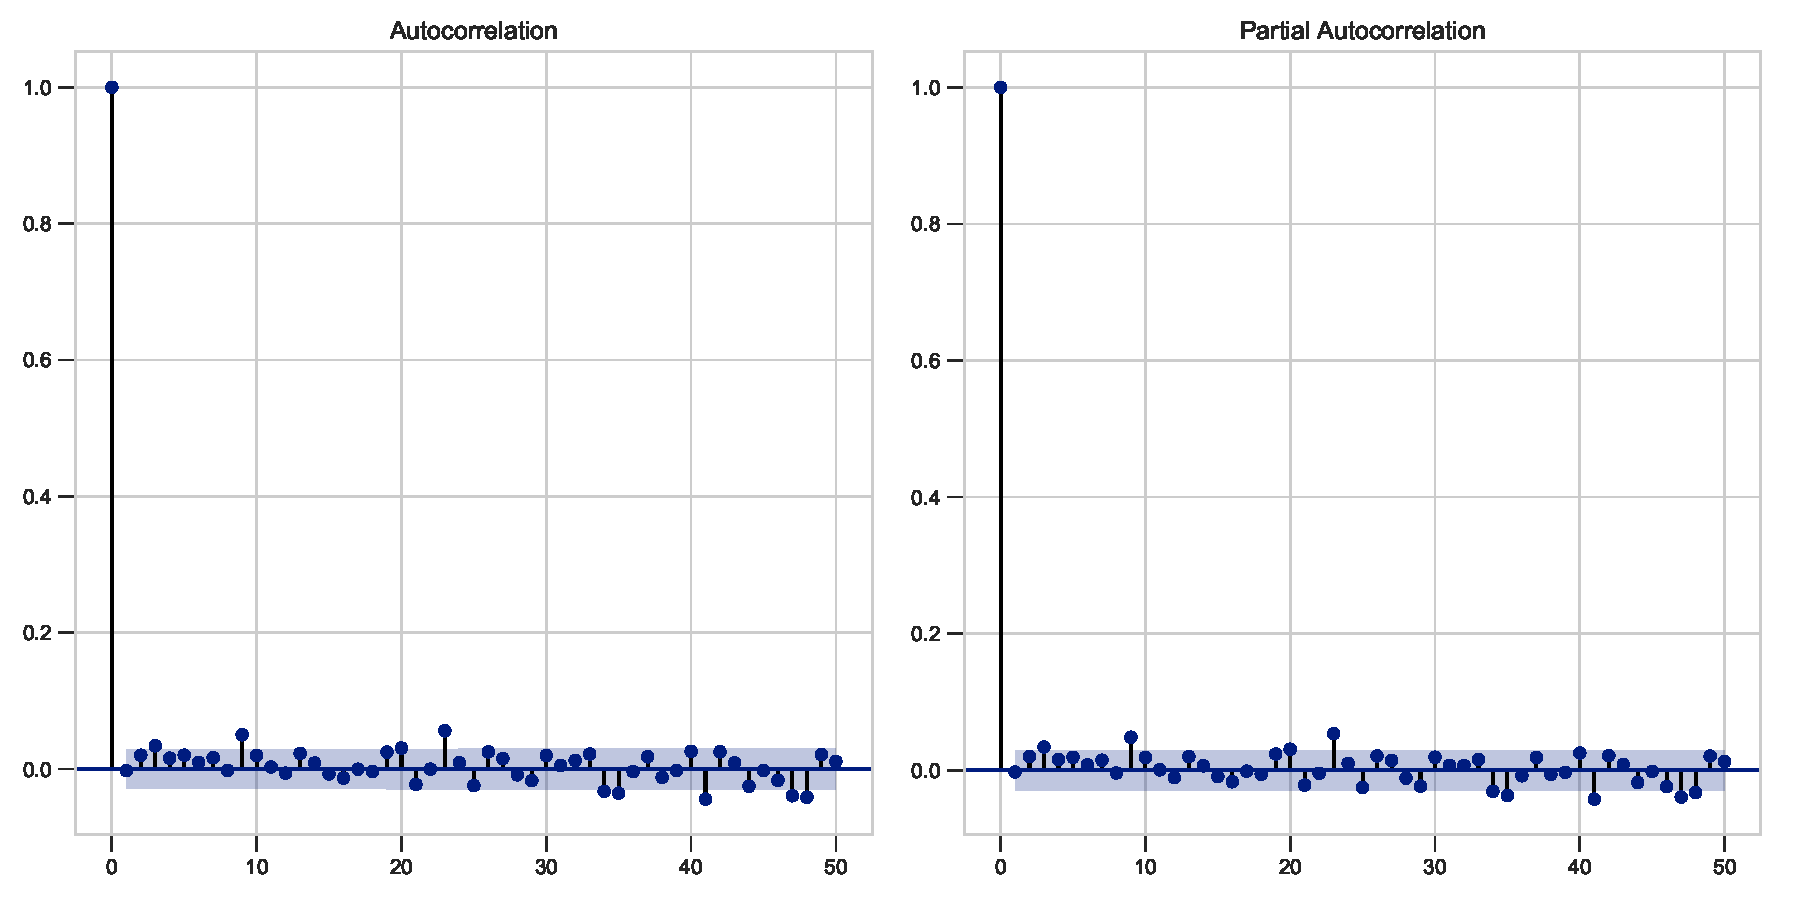
\includegraphics[width=1\columnwidth]{../Figures/sacf_n_spacf_after_reg.pdf}
	\caption{SACF and SPACF of Residuals from Regression Model.}
	\label{fig:sacf_n_spacf_after_reg}
\end{figure}
%

\section{Part 2}
Cross validation RMSE does not improve when information of other currencies are included in to the regression model. Hence they are not used when doing the prediction for the test data.

\end{document}          
